\section{Abstrahierung}

\subsection{Use Cases} 
Die Use Cases (siehe Kapitel \ref{usecases}: Use Cases) sind nach der Nummerierung priorisiert worden. Der UC01 soll auf jeden Fall umgesetzt werden. Der UC02 muss evaluiert werden, ob dies mit der API des DNA Centers im Zusammenspiel mit dem ENCS überhaupt möglich ist. Zu guter Letzt kommt der UC03, welcher nur optional ist und bei genügend verbleibender Zeit implementiert wird.


\subsection{Technologien}
Für das entwickeln des Orchestrierungstool wird Python verwendet. Für das Web Interface wird das Framework Flask eingesetzt. Mit diesen Technologien wird eine Web Anwendung entwickelt, die mit Hilfe der APIs des DNA Centers, des ENCS und der Netzwerkgeräte einzelne Prozesse vereinfacht oder automatisiert.

\subsubsection{Python}
Python ist eine objektorientierte Programmiersprache. Die einfache und leicht erlernbare Python-Syntax hebt die Lesbarkeit hervor und reduziert dadurch die Programmwartung. Python unterstützt Module und Pakete, was die Modularität von Programmen und die Wiederverwendung von Code fördert. Der Python-Interpreter und die umfangreiche Standardbibliothek sind in Quell- oder Binärform kostenlos für alle gängigen Plattformen verfügbar und können frei verteilt werden. \cite{python}

\subsubsection{Flask}
Flask ist ein in Python geschriebenes Webframework. Der Fokus von Flask liegt auf Erweiterbarkeit und guter Dokumentation. Die einzigen Abhängigkeiten sind Jinja2, eine Template-Engine und Werkzeug, eine Bibliothek zum Erstellen von WSGI-Anwendungen. \cite{flask}

\subsubsection{DNA Center Platform}
Cisco hat seit dem Sommer 2018 die DNA Center Platform zur Verfügung gestellt, über die nun auf den API Katalog und andere Ressourcen zugegriffen werden kann. So können beispielsweise die Platform Funktionen auch verwendet werden, um die Bereitstellung und Verwaltung von Netzwerken zu vereinfachen.


So soll das DNA Center nun eine 360 Grad Erweiterbarkeit durch vier verschiedene Platform Funktionen bereitstellen. Dazu gehören die Intent-based APIs, Process adapters, Domain adapters, sowie SDKs. \cite{dnac-platform}

\begin{figure}[H]
	\centering
	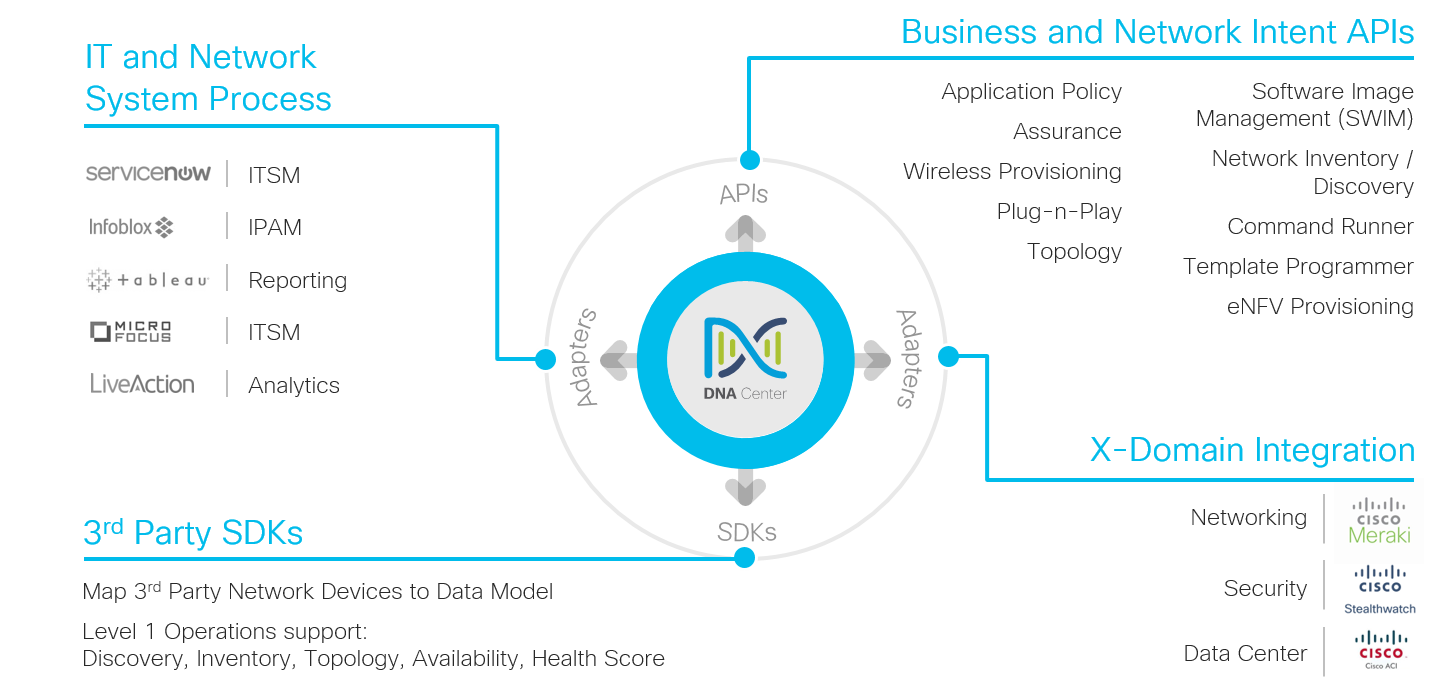
\includegraphics[width=0.8\linewidth]{img/Abstrahierung/dnac-platform}
	\caption{DNA Center Plattform \cite{dnac-platform}}
	\label{fig:DNA Center Plattform}
\end{figure}


\paragraph{Intent-API}

Die Intent-API ist eine Northbound REST API, welche bestimmte Funktionen des DNA Centers verfügbar macht. Mit der RESTful Intent API des DNA Centers können die HTTP- (GET, POST, PUT, DELETE) und JSON-Syntax verwendet werden, um das Netzwerk zu analysieren und zu konfigurieren. \cite{dnac-platform}

Diese APIs findet man im DNA Center unter \textit{Platform $\rightarrow$ Developer Toolkit $\rightarrow$ APIs}

\begin{figure}[H]
	\centering
	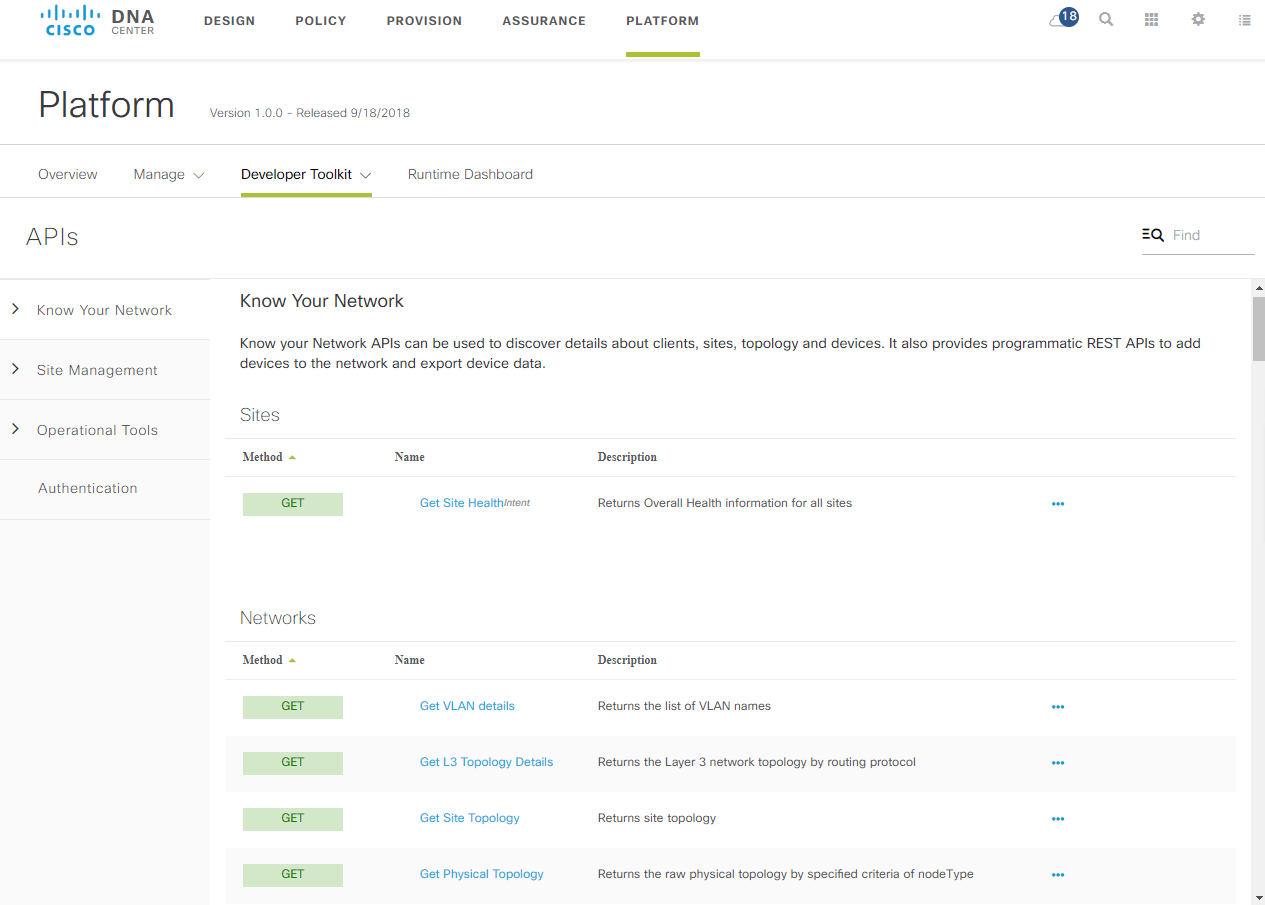
\includegraphics[width=0.8\linewidth]{img/Abstrahierung/dnac-apis}
	\caption{DNA Center Plattform APIs}
	\label{fig:DNA Center Plattform APIs}
\end{figure}

\subsubsection{ENCS/NFVIS API}
Der ENCS beziehungsweise die NFVIS, welche auf dem ENCS läuft, stellt ebenfalls eine programmierbare API für Service Orchestration mittels REST- und NETCONF-API bereit. 

Die API Dokumentationen sind bei NFVIS leider nicht direkt über dessen Applikation verfügbar. Es gibt jedoch eine Dokumentation von Cisco direkt, welche unter dem Namen \textit{API Reference for Cisco Enterprise Network Function Virtualization Infrastructure Software} \cite{nfvis-api} zu finden ist.


\subsection{Umsetzung}

\subsubsection{Ablauf Erstellung Netzwerk}
Um die Erstellung eines Netzwerkes zu vereinfachen, wird ein Wizard erstellt, mit welchem folgende einzelnen Schritte vereinfacht auszuführen sind. 

\begin{figure}[H]
	\centering
	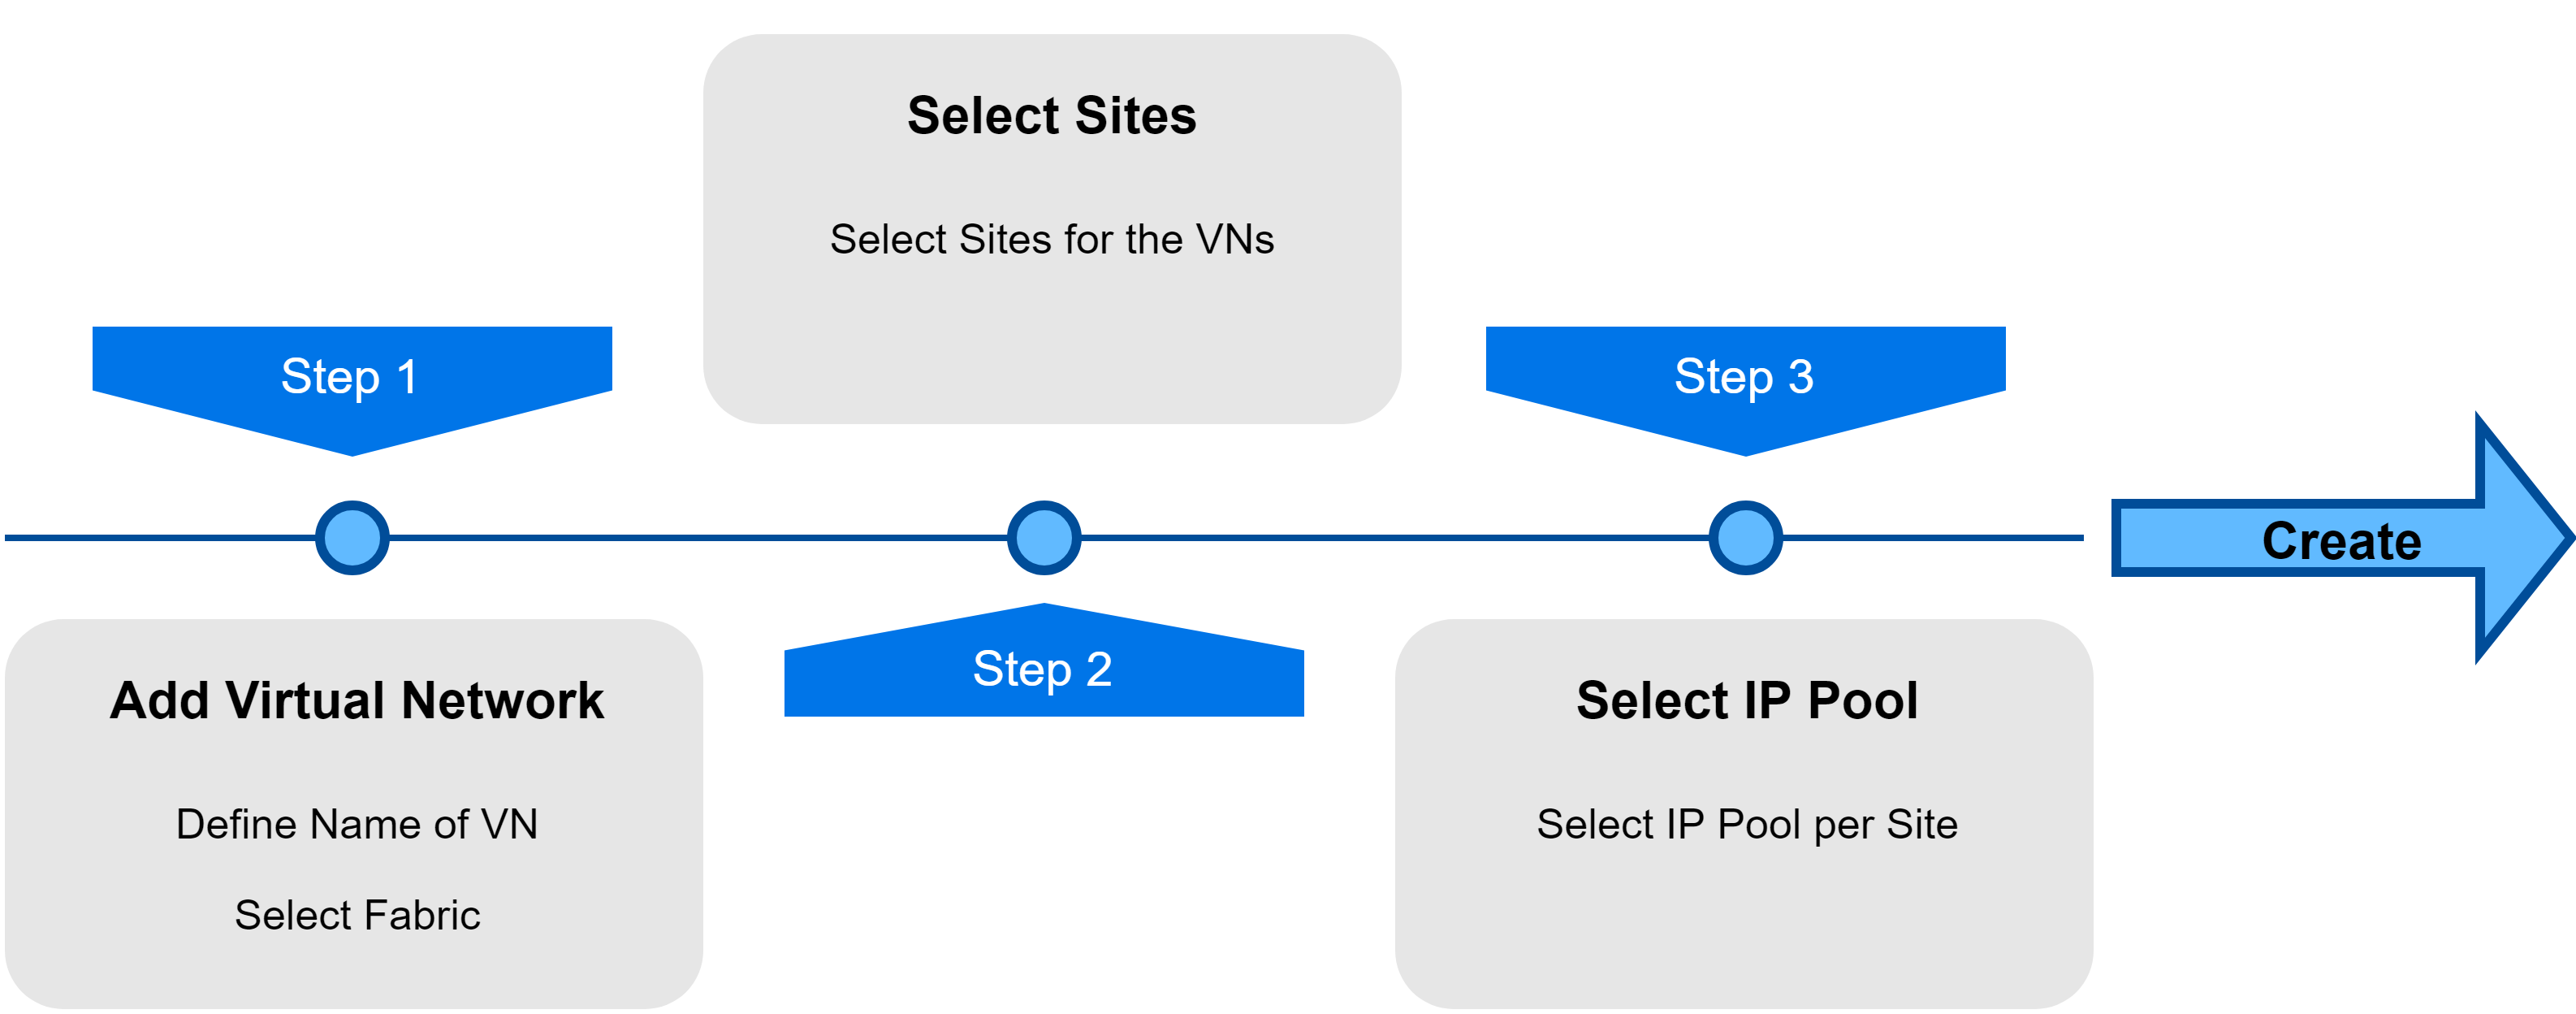
\includegraphics[width=0.8\linewidth]{img/Abstrahierung/addvirtualnetwork}
	\caption{Add Virtual Network}
	\label{fig:Add Virtual Network}
\end{figure}

Um den Wizard zu starten, kann im Orchestrationtool im Home \textit{Virtual Networks $\rightarrow$ Add Virtual Networks} ausgewählt werden. So startet der Wizard mit den in der Abbildung (siehe Abbildung \ref{fig:Add Virtual Network}: Add Virtual Network) aufgezeigten Schritten und man kann Schritt für Schritt die gewünschten Informationen angeben.

Der Wizard verwendet die APIs des DNA Centers, sowie der Netzwerkgeräte. Beim DNA Center mussten teilweise undokumentierte API Endpoints verwendet werden, da die nötigen Funktionen ansonsten nicht verfügbar sind. Dies birgt das Risiko, dass sich diese in Zukunft ändern und die Applikation angepasst werden muss.

\subsubsection{Virtual Machine Management}

Das Virtual Machine Management zeigt alle virtuallen Maschinen auf NFVIS an. Des Weiteren wird der aktuelle Status der VMs, sowie die Netzwerkinterfaces angezeigt. Zudem ist es möglich, eine VM über das Web Interface zu starten oder zu stoppen.

\begin{figure}[H]
	\centering
	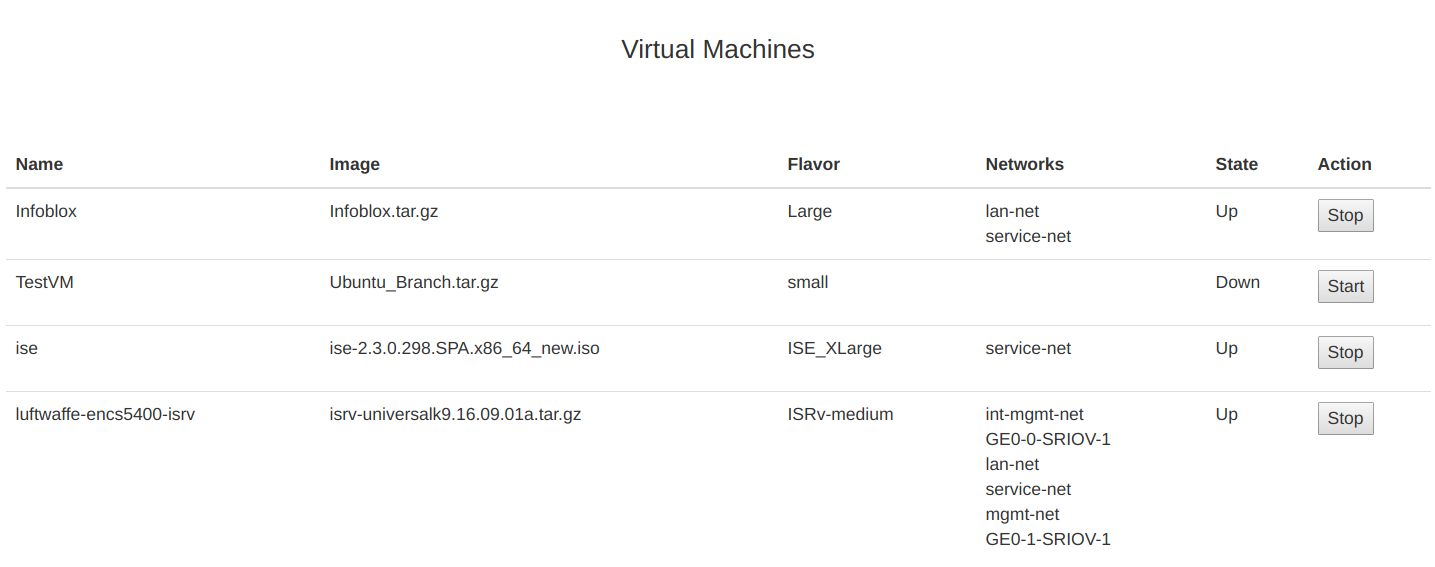
\includegraphics[width=0.8\linewidth]{img/Abstrahierung/vm-management.png}
	\caption{VM Management}
	\label{fig:VM Management}
\end{figure}

\subsubsection{Configuration History}

Dieser Use Case konnte nicht mehr vollständig umgesetzt werden. Derzeit kann nur die aktuelle Konfiguration angezeigt werden. Die Anzeige einer History ist noch nicht implementiert.

\begin{figure}[H]
	\centering
	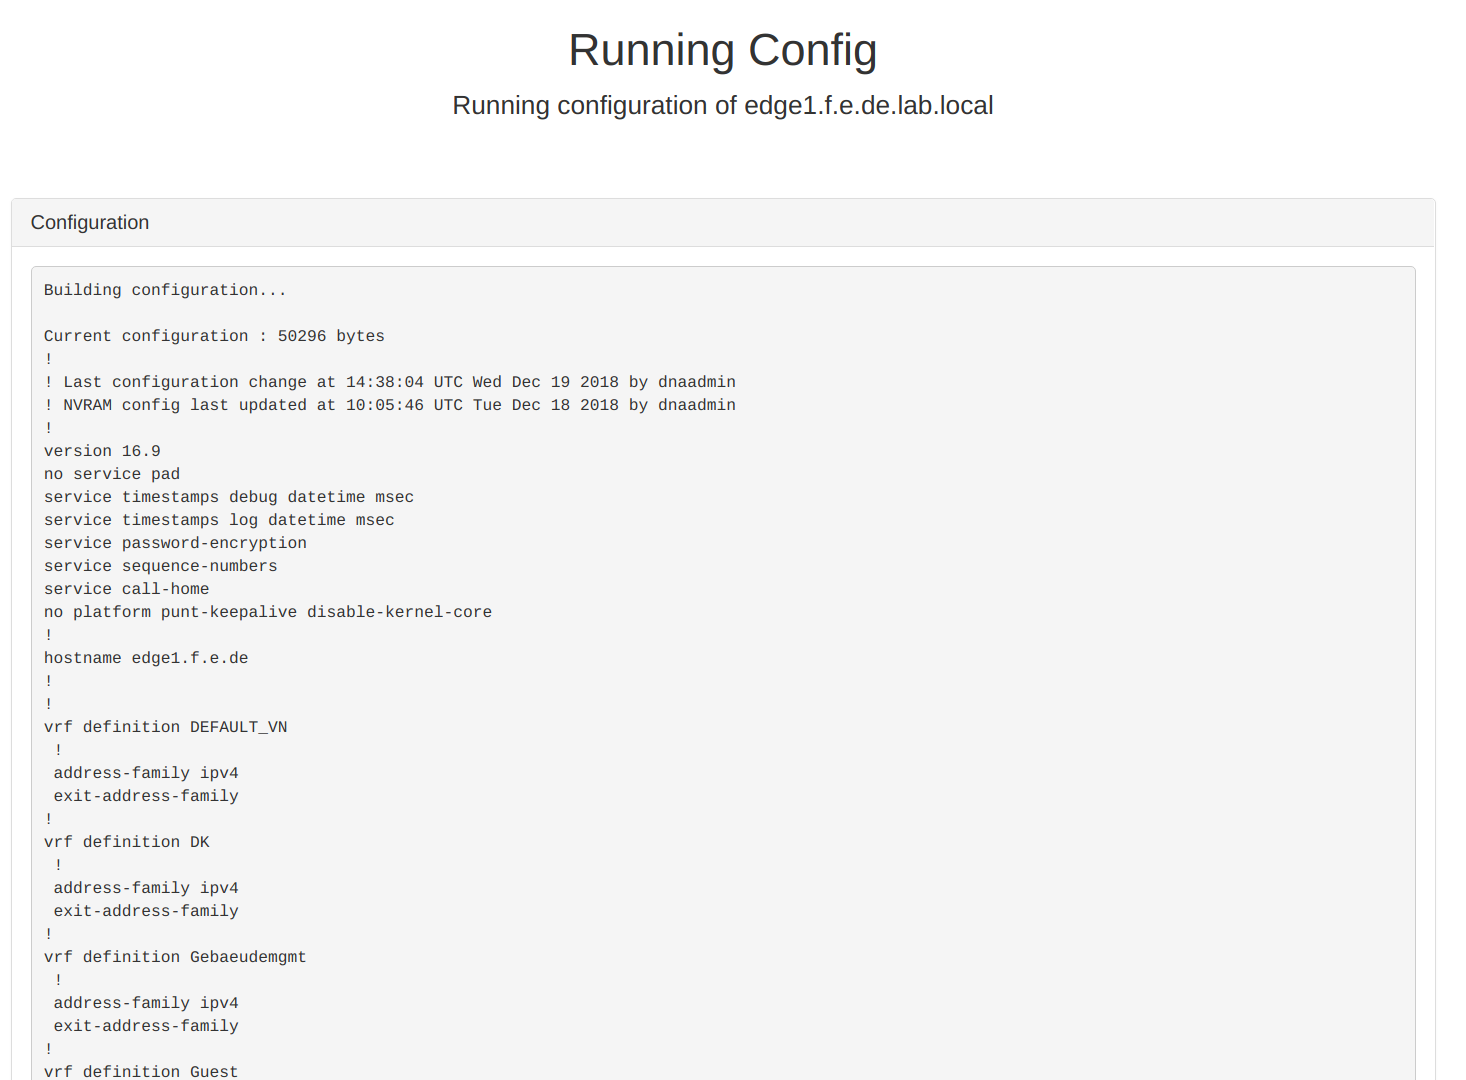
\includegraphics[width=0.8\linewidth]{img/Abstrahierung/running-config.png}
	\caption{Running Config}
	\label{fig:Running Config}
\end{figure}






